% section 3: Models and evaluation method (precision and recall). Comparision among models by f1-score method (show some plots of the main results)
\section{Models}

We tried the following different models:
\begin{enumerate}
	\item Custom Inception Net: a custom version of the Inception\_v1 network;
	\item Custom Resnet: a custom version of the Resnet 101;
	\item Resnet50 (pretrained);
	\item Models with FAST.AI tool.
\end{enumerate}

For each model we will show the comparison between validation and training loss by plotting them. The final models are chosen in the epoch when the validation error is lowest. This is done to avoid overfitting and get the most general solution (early stop).
\subsection{Custom Inception Net}

\begin{figure}[!h]
	\begin{center}
		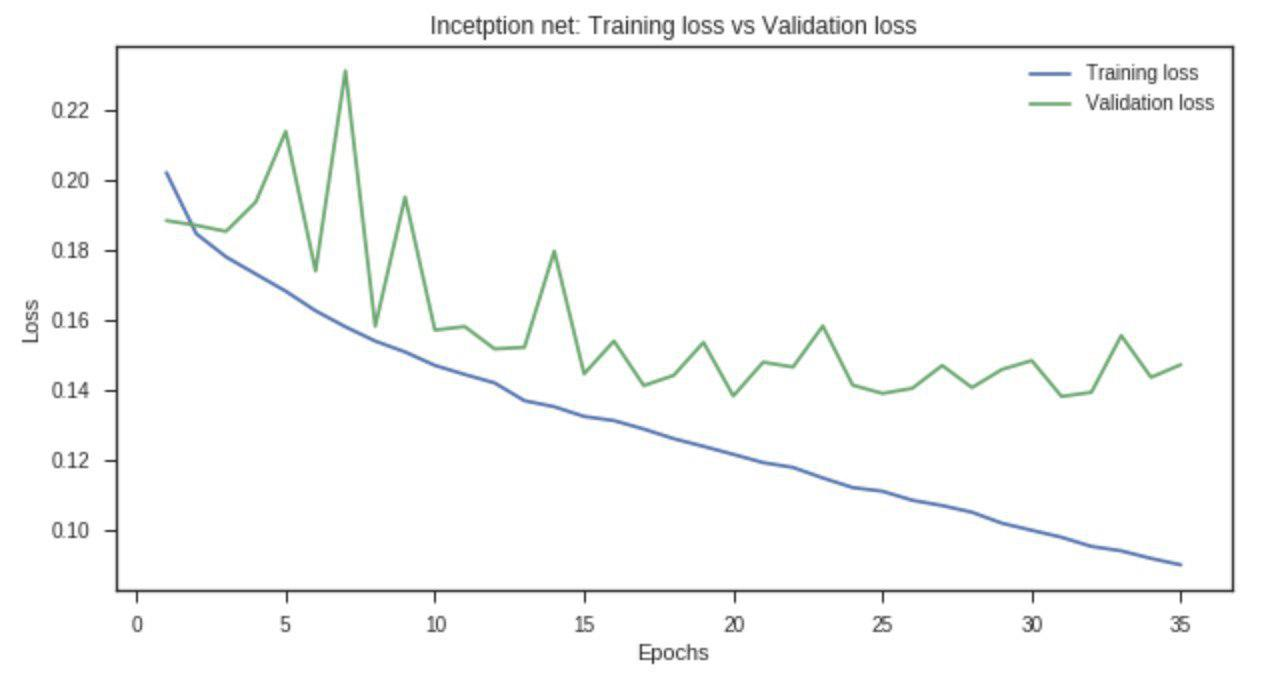
\includegraphics[width=0.5\linewidth]{images/custom_inception_loss.jpg}
		\caption{Custom Inception Net loss}
		\label{fig:cust-incep-loss}
	\end{center}
\end{figure}

The best model was saved at the 32th epoch. The model has been trained for 35 epochs.

\subsection{Custom Resnet}

\begin{figure}[!h]
	\begin{center}
		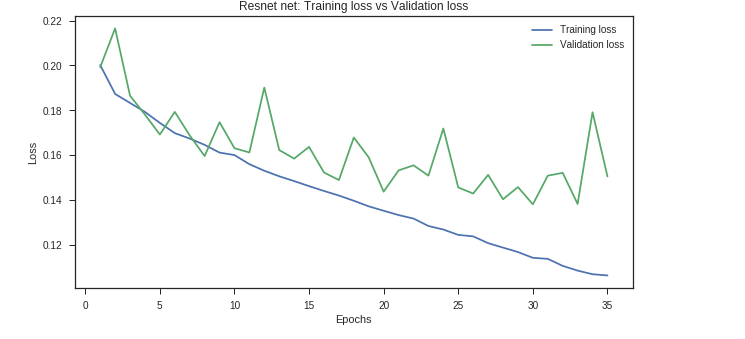
\includegraphics[width=0.6\linewidth]{images/custom_resnet_loss.png}
		\caption{Custom Res Net loss}
		\label{fig:cust-resnet-loss}
	\end{center}
\end{figure}

The best model was saved at the 31th epoch. The model has been trained for 35 epochs.
%\begin{itemize} 
%\item Average loss: 0.1381
%\item precision: 0.34581019077517505
%\item recall: 0.7412008281573499
%\item f1\_score: 0.47159558702453486
%\end{itemize}
\newpage
\subsection{Pretrained Resnet50}

\begin{figure}[!h]
	\begin{center}
		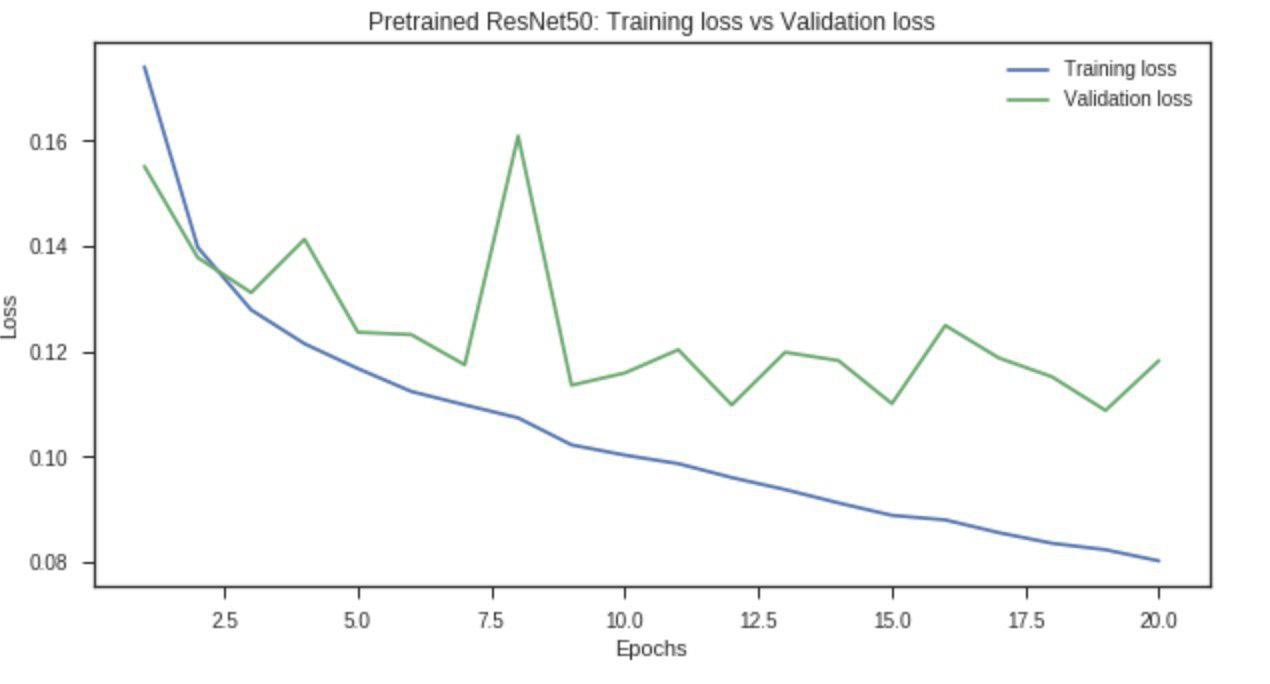
\includegraphics[width=0.5\linewidth]{images/pretrained_resnet50_loss.jpg}
		\caption{Pretrained Resnet50}
		\label{fig:pret-resnet-loss}
	\end{center}
\end{figure}

In the Pretrained Res Net we changed the last fully connected layer in order to have only 14 output neurons. Despite the network was already trained, we freezed the first six layers and we trained the last ones for 20 epoch. The best model was saved at the 19th epoch. So, it seems reasonable assuming that - with more trining epochs - the model can achieve more accurate results.

\subsection{Comparison among the last three models}
We compared the models using the micro-average F1-score on the Validation set:
\begin{enumerate}
	\item F1-score Custom Inception Net: 0.4728875826598089;
	\item F1-score Custom Res Net: 0.47159558702453486;
	\item F1-score Pretrained Res Net: 0.665258711721225.
\end{enumerate}

The best model, according to the micro average F1-score, is the Pretrained Res Net.

\subsection{FAST.AI}

Finally we tried to use the \textbf{fast.ai} deep learning library. This tool is built on top PyTorch and, by using this, we tried two other models: Resnet-18 and Resnet-152. \\
We also attach the code of these two models (as it is explained in section 1). The best one between them is Resnet-18, since it achieves a better micro average f1-score. 
The results are the following:

\begin{itemize}
	\item F1-score of Resnet-18: 0.742385;
	\item F1-score of Resnet-152: 0.724525.
\end{itemize}

%\begin{center}
%	\begin{tabular}{ l | c | c | r }
%		\hline
%		\textbf{Model} & \textbf{accuracy} & \textbf{recall} & \textbf{f1-score}  \\ \hline
%		Inception\_v1 & & & \\
%		Resnet101 & & & \\
%		Inception\_v2 & & & \\
%		\hline
%	\end{tabular}
%\end{center}